\documentclass[11pt]{scrartcl}
\usepackage[letterpaper, portrait, margin=1.0in]{geometry}
\usepackage{lipsum}

\usepackage{colortbl}
\title{Budget Bunny}
\author{Project Specifications Document} % Because it looks so much better than \subtitle{}. Besides, the authors are specified in the version history authors
\date{ }
\usepackage{vhistory}

% Font -- lmodern (Latin Modern Sans)
% LaTeX Font Resource: http://www.tug.dk/FontCatalogue/
\usepackage{lmodern}
\renewcommand*\familydefault{\sfdefault}
\usepackage[T1]{fontenc}

% Item list separation
\usepackage{enumitem}
\setlist{  
	listparindent=\parindent,
	parsep=1pt,
	leftmargin=*,
}

% Referencing and linking
\usepackage{hyperref}

% Colors
\usepackage{color}
\usepackage[dvipsnames]{xcolor}
\definecolor{special-color}{RGB}{51,51,178}

% Images
\usepackage{graphicx}
\graphicspath{{images/}}
\usepackage{subcaption}

% Table
\usepackage{array}
\newcolumntype{L}[1]{>{\raggedright\let\newline\\\arraybackslash\hspace{0pt}}m{#1}}
\newcolumntype{C}[1]{>{\centering\let\newline\\\arraybackslash\hspace{0pt}}m{#1}}
\newcolumntype{R}[1]{>{\raggedleft\let\newline\\\arraybackslash\hspace{0pt}}m{#1}}

% Screen Table
\newcommand{\screentable}[1]{
	\begin{center}
	\begin{tabular}{ |L{5cm} !{\color{lightgray}\vrule} C{3cm} !{\color{lightgray}\vrule} L{7cm}| }
    #1
    \end{tabular}
	\end{center}
}

% Screen Header
\newcommand{\header}[3]{
	\arrayrulecolor{lightgray}\hline
  	\textbf{#1} & \textbf{#2} & \textbf{#3} \\
  	\arrayrulecolor{lightgray}\hline
}

% Screen Row
\newcommand{\row}[3]{
	{#1} & {#2} & {\newline #3 \newline} \\ 
  	\arrayrulecolor{lightgray}\hline
}

% Error Scenarios Table
\newcommand{\errortable}[1]{
	\begin{center}
	\begin{tabular}{ |L{5cm} !{\color{lightgray}\vrule} L{7cm}| }
    #1
    \end{tabular}
	\end{center}
}

% Error Scenarios Header
\newcommand{\errorheader}[2]{
	\arrayrulecolor{lightgray}\hline
  	\textbf{#1} & \textbf{#2} \\
  	\arrayrulecolor{lightgray}\hline
}

% Error Scenarios Row
\newcommand{\errorrow}[2]{
	{#1} & {\newline #2 \newline} \\ 
  	\arrayrulecolor{lightgray}\hline
}

\newcommand{\doublenewline}{
	\newline ~ \newline
}

% All Sections, Subsections, and Subsubsections must have labels so that they can be easily referenced
\newcommand{\bbsection}[2]{
	\section{#1}
    \label{#2}
}
\newcommand{\bbsubsection}[2]{
	\subsection{#1}
    \label{#2}
}
\newcommand{\bbsubsubsection}[2]{
	\subsubsection{#1}
    \label{#2}
}

% Itemize item for core data
\newcommand{\coreitem}[3]{
	\item \textbf{#1} (\textit{#2}): #3 
}

% Use Case Descriptions
\newcommand{\usecase}[8]{
	\begin{description}
    	\item[\textbf{Use Case ID:}] #1
    	\item[\textbf{- Title:}] #2
        \item[\textbf{- Description:}] #3
        \item[\textbf{- Precondition:}] #4
        \item[\textbf{- Postcondition:}] #5
        \item[\textbf{- Main Success Scenario:}] #6
        \item[\textbf{- Extensions:}] #7
        \item[\textbf{- Usage Frequency:}] #8
        \item[]
    \end{description}
}

\begin{document}

\maketitle 
\begin{versionhistory}
	\vhEntry{0.1}{04/10/2016}{Kiefer Yap}{Created the document}
    \vhEntry{0.1.1}{05/11/2016}{Kiefer Yap}{Added Add New Account Screens}
    \vhEntry{0.1.2}{05/29/2016}{Kiefer Yap}{Added View Account Screens}
    \vhEntry{0.1.3}{06/08/2016}{Kiefer Yap}{Added Edit Account Screens}
    \vhEntry{0.1.4}{06/10/2016}{Kiefer Yap}{Added Delete Account Screens}
    \vhEntry{0.1.5}{06/15/2016}{Kiefer Yap}{Added Core Data Section}
    \vhEntry{0.1.6}{06/17/2016}{Kiefer Yap}{Added Use Case Diagram Section}
\end{versionhistory}
\pagebreak

\tableofcontents
\pagebreak

\bbsection{Support Specifications}{support-specifications}

This document is empty at first, but will grow as project features are implemented.  
Screenshots and specific use cases will be specified during the implementation phase.
The localization word list is located in the project's database dump, in the /BudgetBunny/Scripts/output/budget\_bunny.sql file.

\subsection{Hardware}
\begin{description}
\item[iOS Devices:] iPhone and iPad
\item[Device Capabilities:] None
\end{description}

\subsection{Software}
\begin{description}
\item[iOS Version:] iOS 8.1 to 9.3.2
\item[Device Orientations:] Landscape, Portrait, Landscape (Inverted)
\item[Language Support:] English, Japanese, Chinese
\end{description}

\subsection{Development Environment}
\begin{description}
\item[XCode Version:] XCode 7.3.1
\end{description}


\pagebreak

\bbsection{Use Case Diagram}{use-case-diagram-section}

\bbsubsection{Diagram}{use-case-diagram-subsection}
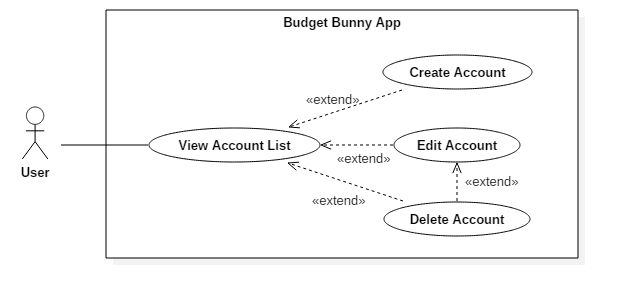
\includegraphics[scale=0.8]{use-case-diagram}

\bbsubsection{Information}{use-case-information}
\pagebreak

\bbsection{Database Schema}{database-schema}

\bbsubsection{Core Data Diagram}{core-data-diagram}
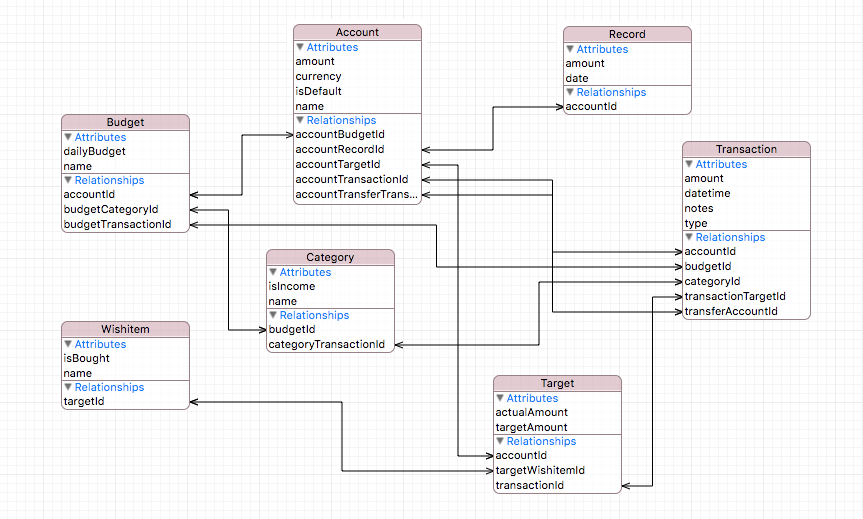
\includegraphics[scale=0.55]{core-data}

\bbsubsection{Model Attributes}{model-attributes}

\bbsubsubsection{Account}{account-attributes}
\begin{itemize}
\coreitem{amount}{double}{Contains the current amount present in the account.}
\coreitem{currency}{string}{Contains the country identifier for the currency used in the account.}
\coreitem{isDefault}{boolean}{If this value is true, then the account is the default account to use for everyday transactions.}
\coreitem{name}{string}{The name of the account.}
\end{itemize}

\bbsubsection{Model Relationships}{model-relationships}

\bbsubsubsection{Account}{account-relationships}
\begin{itemize}
\coreitem{accountBudgetId}{links with the Budget table}{Description to follow once implemented.}
\coreitem{accountRecordId}{links with the Record table}{Description to follow once implemented.}
\coreitem{accountTargetId}{links with the Target table}{Description to follow once implemented.}
\coreitem{accountTransactionId}{links with the Transaction table}{Description to follow once implemented.}
\coreitem{accountTransferTransactionId}{links with the Transaction table}{Description to follow once implemented.}
\end{itemize}
\pagebreak

\section{Application Screens and Use Cases}


\subsection{Adding a New Account}

The Add New Account screen enables users to add a new account by specifying the account's name, currency used and starting balance. The user can also specify whether or not to use this account as the default account to use for everyday transactions.

\subsubsection{Application Screenshots}
\begin{figure}[h]
 
\begin{subfigure}{0.5\textwidth}
  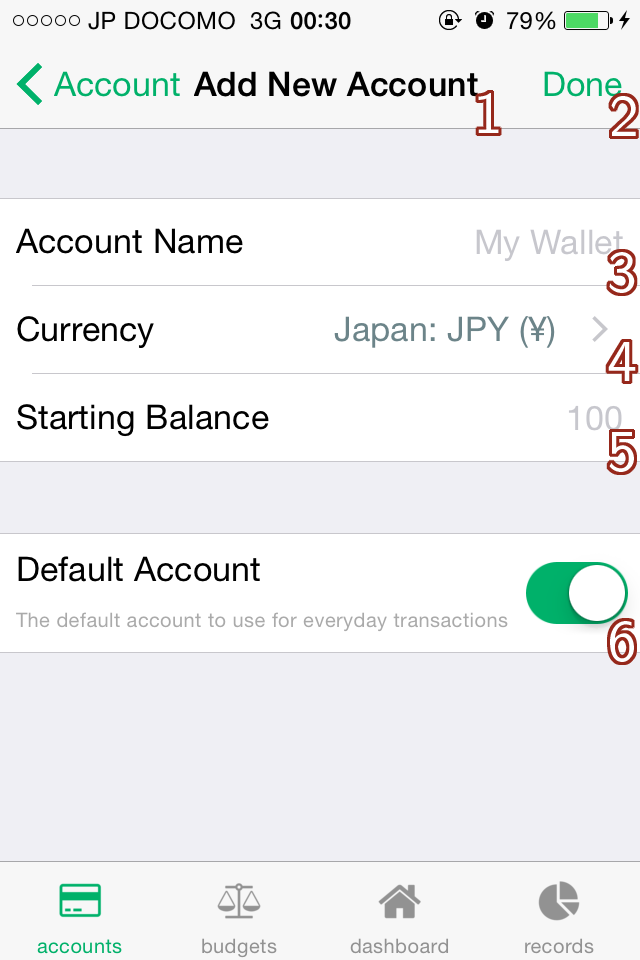
\includegraphics[scale=0.35]{ACC-0001-1} 
  \caption{Add New Account Screen}
  \label{fig:sub-account-1}
\end{subfigure}
\begin{subfigure}{0.5\textwidth}
  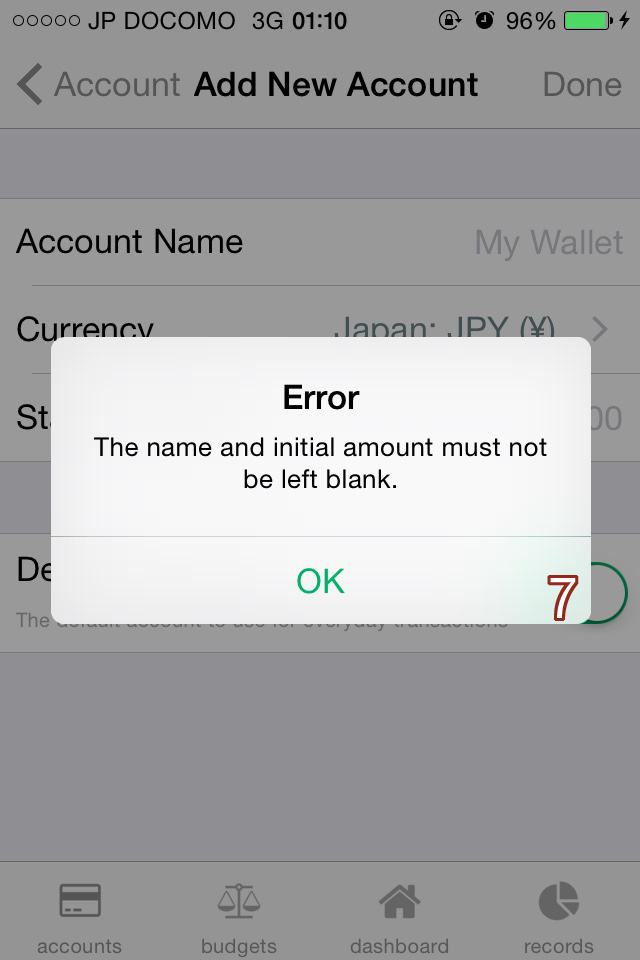
\includegraphics[scale=0.35]{ACC-0001-4}
  \caption{Error Scenario}
  \label{fig:sub-account-2}
\end{subfigure}
 
\caption{Add New Account Screenshots}
\label{fig:account-1}
\end{figure}

\screentable{
	\header{Screen Component}
    	{Type}
        {Description}
    \row{1. Screen Title}
    	{Label Title}
        {Localization Key: MENULABEL\_ADD\_ACCOUNT}
    \row{2. Done Button}
    	{Button}
        {When tapped, the app checks on whether or not both the Account Name and the Initial Amount have been filled. \doublenewline
        If both textfields have been filled, then all fields (that is: account name, currency, initial amount, is default) will be saved into the model. If not, then an error will pop up, prompting the user to have both textfields filled up. \doublenewline
        Localization Key: BUTTON\_DONE
        } 
    \row{3. Account Name Cell}
    	{Table Cell}
        {This table cell consists of two UI elements: A label and a textfield. \doublenewline
        
        Tap anywhere in the cell and the textfield will be placed in focus, bringing up a QWERTY keyboard. Tap anywhere outside the cell to dismiss the keyboard. \doublenewline
        
        The textfield has a character limit of 25 characters. This is because the average word has an average of five letters, and a four-word account name suffices.\doublenewline
        
        Localization Keys: LABEL\_NAME, TEXTFIELD\_NAME\_PLACEHOLDER} 
    \row{4. Currency Cell}
    	{Table Cell}
        {This table cell consists of two label UI elements. \doublenewline
        
        When this table cell is tapped, the cell will be briefly filled with a light green background, then fade out as the screen transitions to the Currency Selection screen. The default currency depends on the user's device locale.\doublenewline 
        
        Localization Key: LABEL\_CURRENCY} 
}

\screentable{
	\header{Screen Component}
    	{Type}
        {Description}
    \row{5. Initial Amount Cell}
    	{Table Cell}
        {This table cell consists of two UI elements: A label and a textfield. \doublenewline
        
        Tap anywhere in the cell and the textfield will be placed in focus, bringing up a keyboard that is numeric with a decimal point.  Tap anywhere outside the cell to dismiss the keyboard. \doublenewline
        
        The textfield has a character limit of 22 characters. This is because the largest banknote ever released due to hyperinflation has a value of ${10}^{20}$.\doublenewline
         
        Localization Keys: LABEL\_STARTING\_BALANCE, TEXTFIELD\_STARTING\_BALANCE\_ PLACEHOLDER} 
    \row{6. Default Account Cell}
    	{Table Cell}
        {This table cell consists of three UI elements: two labels and a switch. \doublenewline
        
        Tap anywhere in the cell and the switch will be toggled. \doublenewline
        
        Localization Keys: LABEL\_IS\_DEFAULT\_ACCOUNT, LABEL\_IS\_DEFAULT\_ACCOUNT\_ DESCRIPTION} 
    \row{7. Error Alert}
    	{Alert Controller}
        {This alert controller has two labels. \doublenewline
        
        The alert is displayed when either the account name or the initial amount has not been filled, and the user taps "Done". \doublenewline
        
        Localization Keys: ERRORLABEL\_ERROR\_TITLE, ERRORLABEL\_NAME\_CURRENCY\_ NOT\_EMPTY}
}

\subsubsection{Use Cases}


\subsection{Currency Selection}

The currency selection screen enables users to search and select a currency to use for their new account. The user can search for the country's name, the currency name, or the currency symbol. Once the user is satisfied with their selection, they can tap the Back button to return to the Add New Account screen, where they will see their newly selected currency in the Currency Cell (See Figure 1, \#4).

\subsubsection{Application Screenshots}
\begin{figure}[h]
 
\begin{subfigure}{0.5\textwidth}
  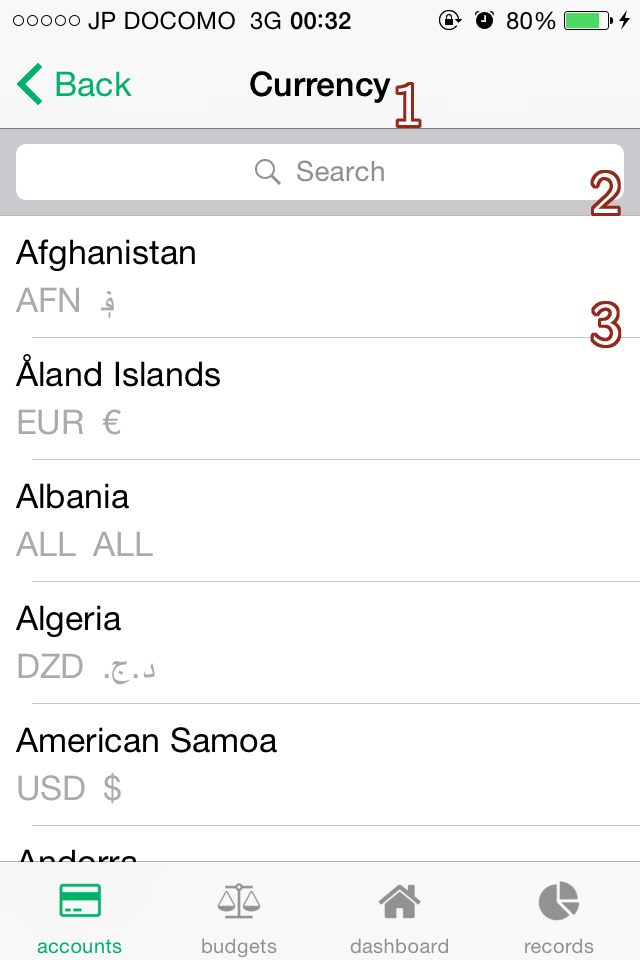
\includegraphics[scale=0.35]{ACC-0001-3} 
  \caption{Currency Selection Screen}
  \label{fig:currency-1}
\end{subfigure}
\begin{subfigure}{0.5\textwidth}
  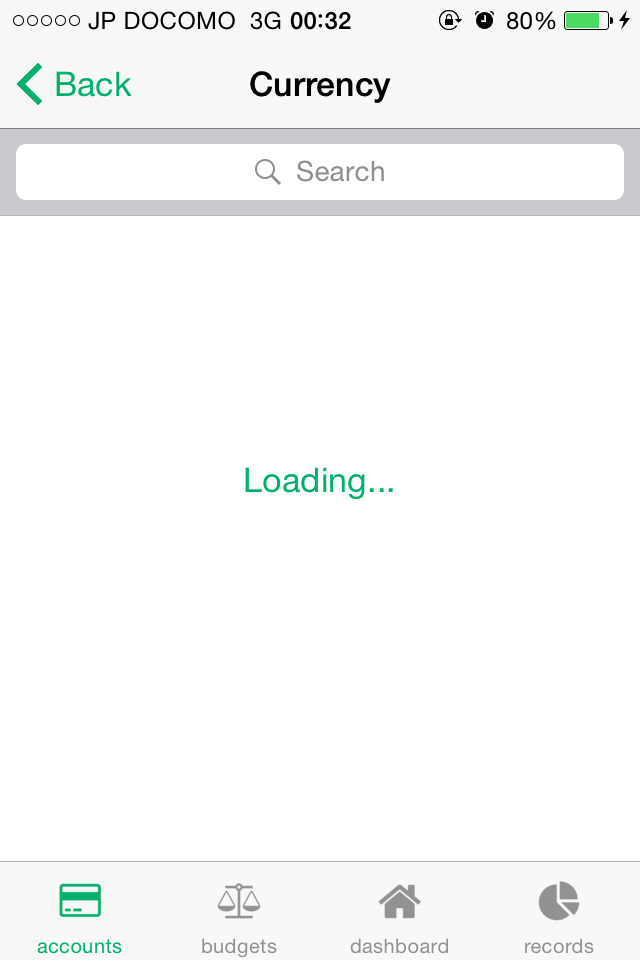
\includegraphics[scale=0.35]{ACC-0001-2}
  \caption{Currency Loading Screen}
  \label{fig:currency-2}
\end{subfigure}
\caption{}
\label{fCurrency Selection Screenshots}
\end{figure}

\screentable{
	\header{Screen Component}
    	{Type}
        {Description}
    \row{1. Screen Title}
    	{Label Title}
        {Localization Key: MENULABEL\_CURRENCY\_PICKER}
    \row{2. Search Field}
    	{Search Bar}
        {When tapped, a QWERTY keyboard is displayed, and the search textfield is given focus. \doublenewline
        
        At the same time, the width of the textfield shortens, giving way to the Cancel button which, when tapped, dismisses the keyboard and returns it to the state shown in the screenshot. 
        } 
        
    \row{3. Currency Selection Cell}
    	{Table Cell}
        {This table cell consists of three UI labels showing the currency's country, code, and symbol. \doublenewline
        
        Tap anywhere in the cell and a checkmark will appear on its right side, indicating that a type of currency has been selected.
        } 
        
    \row{4. Loading Screen}
    	{Label}
        {This label is displayed while the currency data is being loaded. \doublenewline
        
        While loading, the user cannot scroll or type in the search bar.\doublenewline 
        
        Localization Key: LABEL\_LOADING} 
}

\subsubsection{Use Cases}
\pagebreak

\end{document}